\chapter{Results \& Discussion}\label{ch:results}

\section{Results}

\subsection{Which Synthesis Method Is Better?}

\subsection{Did we manage to achieve what we wanted?}
\begin{itemize}
\item do we think we are successful?
\item did we manage to do what we wanted?
\item did we prove what we wanted to prove?
\item is it really a useful tool?
\item who is it targeting as a user?
\end{itemize} 

\section{What did we do new?}
Combined all three major sounds inside a game or an application (impact, rolling, scratching) and made them available and ready-to-use to developers.

\section{Discussion}

\subsection{Types of games that it can be used}
This tool can be used for development of all sorts of games that include object interaction. They can vary from indoor AR applications to open world environment games running in consoles. 

\subsection{Why our work can be used in VR/AR?}


\subsection{CPU demands}
Synthesizing sounds for applications real-time instead of using a mass of prerecorded clips is a good solution to the storage problem of nowadays portable and limited in memory devices. On the other hand, it is challenging and requires a lot of CPU performance when usually audio is restricted to a low limit and most of it is given to graphics, physics and artificial intelligence (AI) \cite{lloyd2011sound}. 

In our tool, however, when profiling a demonstration of a wine bottle rolling down a number of oblique platforms (seen in figure \ref{fig:test_sc2}), using the \textit{Profiler Window} of Unity Editor we can see that except for the initialization at the beginning where scripts consume some CPU power, the rest of the demonstration remains stable in performance and around $100 fps$ (figure \ref{fig:profile}). This performance test was held on a laptop with 4 Intel\textregistered\ Core\texttrademark\ i7-6700HQ CPUs running at 2.60GHz, each with 2 hardware threads.

\begin{figure}[H]
  \centering
    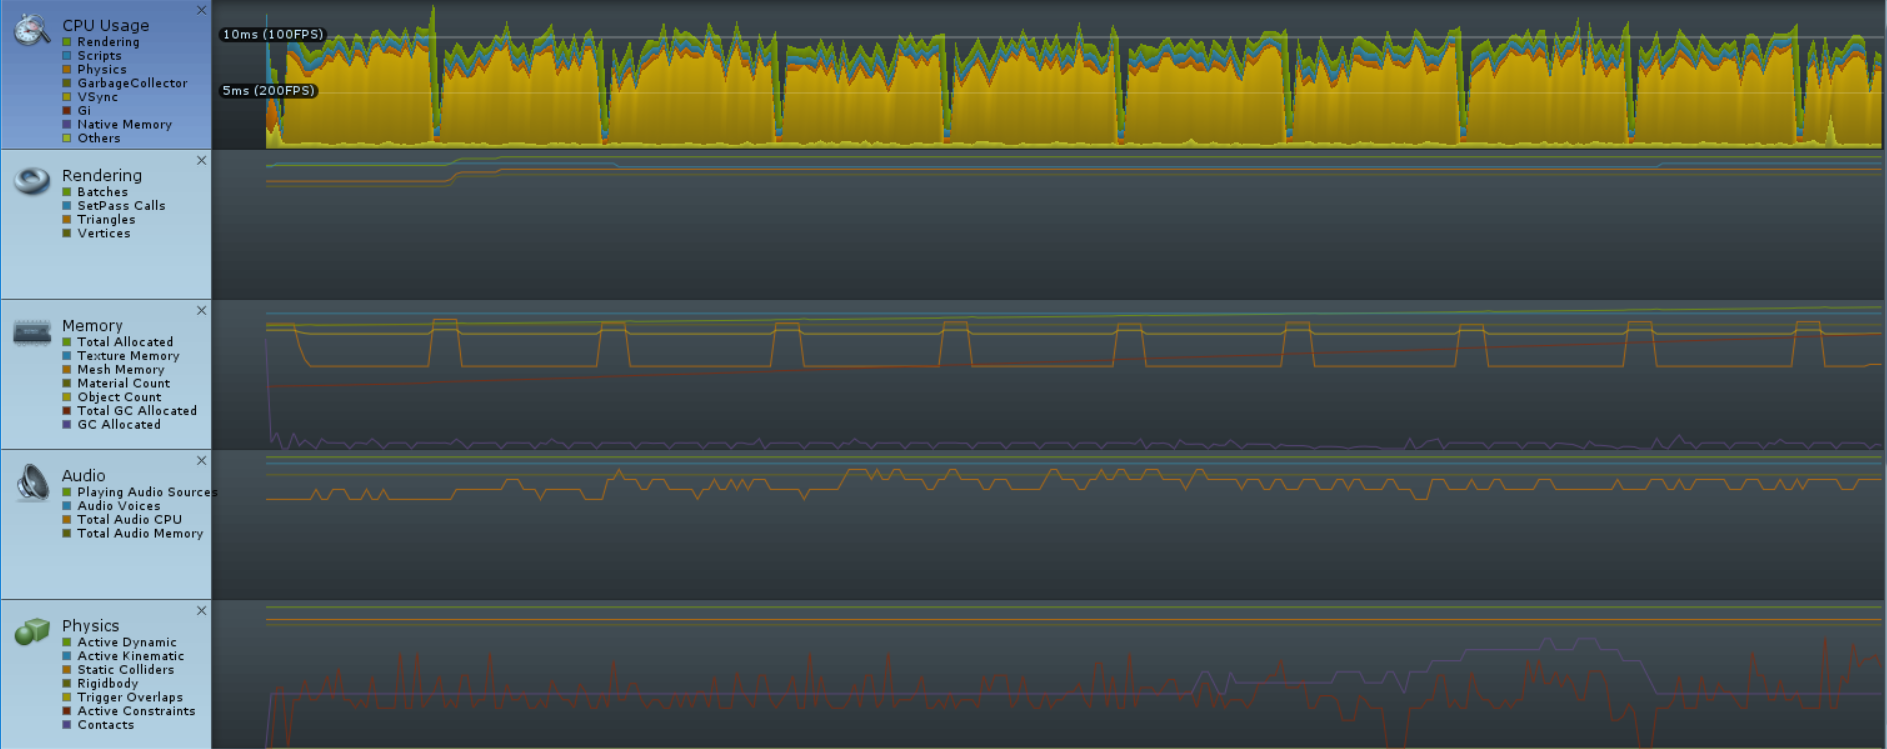
\includegraphics[width=0.9\textwidth]{profiling1.PNG}
      \caption{The profiler view of Unity Editor when a wine bottle rolls down a number of platforms.}
      \label{fig:profile}
\end{figure} 

\Todo{demo with a lot of objects and check if it needs to reduce quality}

\subsection{Bugs}
\begin{itemize}
\item you have to press apply on prefabs
\item the procedure of putting the freq and ampl data in
\item it is object specific (not a bug actually, more like a drowback)
\item lack of acoustical richness that might characterize synthetic signals \cite{giordano2006material}
\item some objects are not modal
\end{itemize}

\subsection{How can we improve our work?}
\begin{itemize}
\item take into account the environment (reverberation etc)
\item make objects destructible
\item randomize initial phase so peaks of the sine wave don't line up and distort the sound (saturation)
\end{itemize}

\subsection{Pros and Cons of Procedural Game Audio}